% !TEX root = Nies_Lukas_BSc_Thesis_SiPM.tex

\chapter{Particle interaction with matter} \label{ch:particles}

As numerous kinds of particles exist as diverse are their types of interaction with matter. To classify this, one not only has to consider the particles' mass, charge and energy but also their behavior due to interaction through the fundamental forces. To describe some of the most essential interactions, a brief overview is given in the following.      

\section{Interaction of photons}

The photon is a neutral and massless particle. As the force carrier of the electromagnetic force the photon interacts electromagnetically. Since photons have no mass they always move with the speed of light. Their energy is given by the product of the Planck constant $h$ and the frequency $\nu$
\begin{align}
E=h\cdot\nu=h\cdot\frac{c}{\lambda},
\end{align}
where $\lambda$ is the corresponding wavelength. The interaction of these particles depends on their energy, the different types are shown in figure \ref{fig:ch1:photons}.\par 
Photons with low energy (long wavelength) do elastic scattering with electrons (\textit{compton scattering}). In this process they are deflected by an angle $\vartheta$ and lose energy, $E_{\gamma}'$, to the electron. This mechanism leads to an increase of wavelength 
\begin{align}
\Delta\lambda=\frac{h}{m_ec}\left(1-\cos(\vartheta)\right)=\lambda_c\left(1-\cos(\vartheta)\right) \label{eq:compton_wavelength},
\end{align}
where $m_e$ is the mass of an electron and $\lambda_c$ is the so called \textit{compton wavelength}. It can be seen that the energy deposit at $\vartheta=180\degree$ is largest. The energy gain of the electron is given by 
\begin{align}
E_e'=E_\gamma-E_\gamma'=E_\gamma\left(1-\frac{1}{1+\frac{E_\gamma}{m_ec^2}\left(1-\cos(\vartheta)\right)}
\right).
\end{align} \\[0.5cm] 
\par 
\begin{figure}[t]
	\floatbox[{\capbeside\thisfloatsetup{capbesideposition={left,center},capbesidewidth=5cm}}]{figure}[\FBwidth]
	{\caption[Interaction of phtonos with matter]{Energy dependency of the attenuation coefficient $\mu/\rho\sim\sigma$ in lead \cite{povh}. The cross section rises suddenly when the photon-energy is high enough to excite an inner shell. A more detailed version can be found in figure \ref{ap:A:photons_detailed}.}    
	\label{fig:ch1:photons}}
	{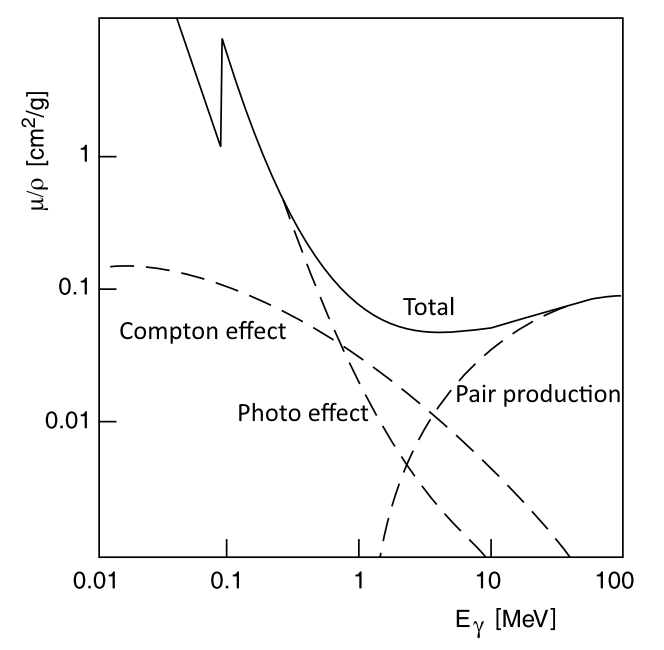
\includegraphics[width=0.6\textwidth]{./graphics/ch1/photo_absorption.png}}
\end{figure}
When it comes to higher energies the \textit{photoelectric effect} comes into play. It describes the entire absorption of a photon by an atomic shell where the absolute photon-energy $E_\gamma$ is transferred to an electron with binding energy $E_B$
\begin{align*}
h\nu + \text{atom} = \text{atom}^{+}+e^{-}.
\end{align*} 
The electron gets unbound when $E_\gamma>E_B$ and the atom gains momentum through the recoil which is small due to its high mass. For higher energies, electrons from inner shells (K,L,M,...) can be removed, too. This mechanism is favored since the cross section for these processes is high when $E_\gamma-E_B$ is low \cite{wermes}. This generates a higher cross section for inner shells which is visualized by a sudden rise in figure \ref{fig:ch1:photons}.\par 
\textit{Pair production} is possible when the photon energy exceeds twice the electrons' invariant mass ( $E_\gamma\gtrsim 2m_ec^2\approx\SI{1.02}{\MeV}$ ): the photon converts into an electron-positron-pair in an external electromagnetic field. As before, the recoil energy can be neglected. This process is dominating for very high energies.\par 
All these mechanisms lead to a scattering or an absorption of photons. This loss of particles is described by \textit{Beer-Lambert's Law}
\begin{align}
N(x)&=N_0e^{-\mu x}=N_0e^{-\frac{x}{\lambda}}, 
\label{eq:beer_lambert}
\end{align} 
where $N_0$ is the initial number of particles in a photon beam, $\mu$ the attenuation coefficient and $\lambda$ the mean free path between collisions. The formula can be derived by shifting and integrating the definition of the attenuation coefficient which illustrates the ability of a material to absorb photons:
\begin{align}
\mu=-\frac{1}{N}\dv{N}{x}=\rho\frac{N_A}{A}\sigma=n\sigma=\frac{1}{\lambda}.
\end{align}
It can be seen that the absorption of photons depends on the materials' density $\rho$ and mass number $A$, $N_A$ is the \textit{Avogadro number}. 

\section{Interaction of charged particles}

A heavy charged particle interacting with matter loses energy through excitation and ionizing processes. These \text{ionization losses} can be expressed by the \textit{Bethe-Bloch formula}, which gives the \textit{stopping power} $S=-\dv{E}{x}$ of particles in matter: 
\begin{align}
-\langle\dv{E}{x}\rangle=\frac{4\pi}{m_ec^2}\frac{nz^2}{\beta^2}\left(\frac{e^2}{4\pi\epsilon_0}\right)^2\left[\ln\frac{2m_ec^2\beta^2}{I\cdot(1-\beta^2)}-\beta^2\right].
\label{eq:bethe_bloch}
\end{align}
\begin{center}
	\centering
	\small
	$ze$ and $\beta=\frac{v}{c}$: charge and velocity of incident particle, $I$ and $n$: mean ionization potential and electron density of the matter 
\end{center}
This equation approximates the mean energy loss d$E$ per length d$x$ in an area of $0.1<\beta\gamma<1000$ \cite{PDG}. This correlation is shown in figure \ref{fig:ch1:bethe_bloch}. The energy loss for small momenta is large since the interaction time is longer for slow particles. The graph decreases with $1/\beta^2$ for greater energies and reaches a minimum at approximately $\beta\gamma=3-4$. At this point the so called \textit{minimum ionizing particles (MIP)} dissipate roughly 2 $\si{\MeV\per\gram\per\square\centi\meter}$. A relativistic rise with almost $\sim\ln(\gamma)$ follows for growing $\beta\gamma$ due to rare large energy transfers to few electrons \cite{PDG}. \par 
\begin{figure}[b]
	\floatbox[{\capbeside\thisfloatsetup{capbesideposition={right,center},capbesidewidth=5cm}}]{figure}[\FBwidth]
	{\caption[Interaction of charged particles with matter]{Normalized energy loss of particles in different targets \cite{povh}. The x-axis shows the particle energies in $\beta\gamma=p/mc$. Again, a more detailed version can be found in figure \ref{ap:A:bethe_bloch_detailed}.}    
		\label{fig:ch1:bethe_bloch}}
	{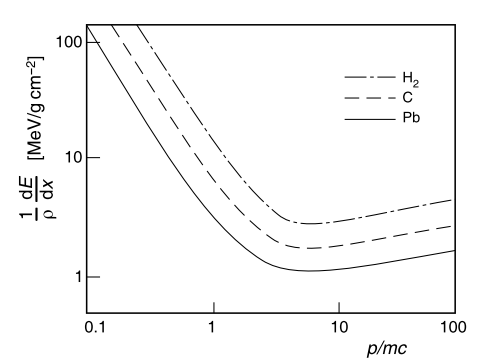
\includegraphics[width=0.6\textwidth]{./graphics/ch1/bethe_bloch.png}}
\end{figure}
Due to their small mass, electrons mainly lose energy by emitting \textit{brems\-strah\-lung} when decelerated in an electromagnetic field of a nucleus. These \textit{radiation losses} depend on the effective nuclear charge $Z_{\text{eff}}^2$ due to shielding effects of bound electrons and the concentration $n$ of electrons in the solid \cite{rodnyi}
\begin{align}
-\dv{E}{x}=Z_{\text{eff}}^2\cdot nE_0, 
\label{eq:energy_loss_electrons}
\end{align}  
where $E_0$ is the energy of the incident electron. \par   
\begin{figure}[t]
	\floatbox[{\capbeside\thisfloatsetup{capbesideposition={left,center},capbesidewidth=5cm}}]{figure}[\FBwidth]
	{\caption[Interaction of electrons with matter]{Energy loss of electrons in silicon. Ionization processes are dominating for low energies. The intersection of the dashed lines gives the critical energy above bremsstrahlung influences most. The dotted curve shows the Bethe-Bloch-like behavior of protons as comparison. Amended from \cite{wermes}.}    
		\label{fig:ch1:electrons}}
	{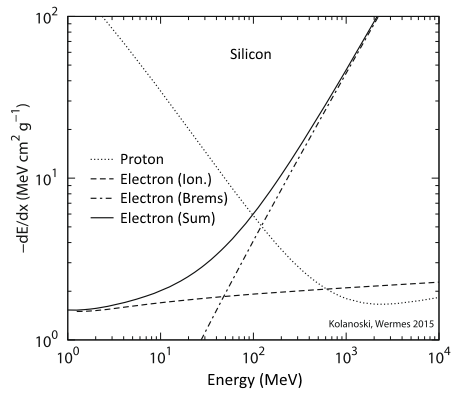
\includegraphics[width=0.6\textwidth]{./graphics/ch1/energy_loss_electrons.png}}
\end{figure}
Ionization losses caused by \tit{coulomb scattering} dominate at lower energies. The \tit{critical energy} gives the energy where radiation losses become the dominant process. It can roughly be estimated by 
\begin{align}
E_c\approx\frac{800}{Z_{\text{eff}}},
\label{eq:radiation_length}
\end{align}
given in $\si{\MeV}$ \cite{rodnyi}. Figure \ref{fig:ch1:electrons} illustrates the energy loss of electrons in silicon, the critical energy is given by the intersection of the dashed lines. A \textit{radiation length} $X_0$ can be formulated analog to $\lambda$ in formula \eqref{eq:beer_lambert}. \par 
Due to bremsstrahlung, incident high energy electrons produce photons with sufficient energy to create electron-positron-pairs. These secondary products have enough energy to produce even more particles. The resulting \textit{electromagnetic shower} only stops when the energy of the cascade electrons falls below the critical energy \cite{rodnyi}. The \textit{Moli\`{e}re radius} can be approximated by
\begin{align}
R_M=\frac{21X_0}{E_c}
\label{eq:moliere} 
\end{align}
and provides an estimation of the transversal geometry of a defocussing, cone-like shower. This relation also applies to high energy photons.        

\section{Interaction of hadrons}
Neglecting the electromagnetic interaction, the interplay of hadrons (p,n,$\pi$,K,...) with matter is hard to calculate since the strong force knows many different interaction processes. To give a short qualitative approach, one can define a \textit{hadronic interaction length}  
\begin{align}
\lambda_a=\frac{A}{N_A\rho\sigma_{\text{in}}}\propto A^{-\frac{2}{3}}
\end{align}
analogous to the relations \eqref{eq:beer_lambert} and \eqref{eq:radiation_length}, where $\rho\sim A$ is the materials' density and $\sigma\sim A^{\frac{2}{3}}$ is the cross section for inelastic scattering \cite{wermes}. \par 
Neutrons as the most prominent uncharged hadron interact via scattering and absorption with nuclei. Inelastic scattering is favored for higher energies ($\sim \SI{10}{\MeV}$). For lower energies, elastic scattering and absorption are likely. Both processes excite the nuclei which then emit a photon. This is important when it comes to moderating hot neutrons to receive cold (low energy) neutrons. 